\documentclass[11pt]{amsart}

% packages

\usepackage{amsfonts, amsthm, amssymb, amsmath, stmaryrd, etoolbox, mathtools}
\usepackage{graphicx,caption,subcaption}
\usepackage{tikz}
\usetikzlibrary{matrix,arrows}

% new commands

\newcommand{\RR}{\mathbb{R}}
\newcommand{\ZZ}{\mathbb{Z}}
\newcommand{\NN}{\mathbb{N}}
\newcommand{\QQ}{\mathbb{Q}}
\newcommand{\CC}{\mathbb{C}}
\newcommand{\from}{\colon}
\newcommand{\defn}[1]{\textbf{#1}}
\newcommand{\tin}{\colon}

% fonts

\newcommand{\cat}[1]{\mathbf{#1}}
\newcommand{\type}[1]{\mathtt{#1}}

% math operators

\DeclareMathOperator{\Hom}{Hom}
\DeclareMathOperator{\id}{id}
\DeclareMathOperator{\ob}{Ob}
\DeclareMathOperator{\arr}{arr}
\DeclareMathOperator{\im}{im}
\DeclareMathOperator{\Aut}{Aut}
\DeclareMathOperator{\Bij}{Bij}
\DeclareMathOperator{\Sub}{Sub}

%%%%%%%%%%%%%
% begin document
%%%%%%%%%%%%%
\begin{document}

\title{Notes on a pushout of sets}
\maketitle

%%%%%%%%%%%%%
% new section
%%%%%%%%%%%%%
\section{the setup}

The idea is that we have types $A$, $B$, and $C$, all of which are sets. 
The question: is the pushout given by the square
\[
	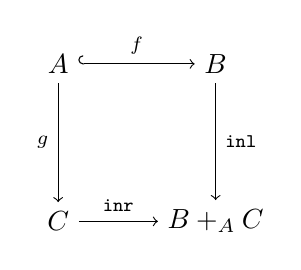
\begin{tikzpicture}
		\node (C) at (0,0) {$C$};
		\node (BAC) at (2,0) {$B +_A C$};
		\node (A) at (0,2) {$A$};
		\node (B) at (2,2) {$B$};
		\draw[right hook ->]  (A) to node [above] {\scriptsize $f$} (B);
		\draw[->]  (A) to node [left] {\scriptsize $g$} (C);
		\draw[->]  (B) to node [right] {\scriptsize $\type{inl}$} (BAC);
		\draw[->]  (C) to node [above] {\scriptsize $\type{inr}$} (BAC);
	\end{tikzpicture}
\]
also a set when $f$ is a monomorphism?

Recall that a \defn{set} is a type such that, 
for any elements $x$, $y$ and $p$, $q \from x = y$, 
we have $p = q$.  
Thus to determine whether $B +_A C$ is a set,
we need to access its identity types.  
We do this with an \emph{encode-decode} style proof.  

Roughly, a proof of this sort begins by guessing
what the identity types are.  That is,
for each $x$ and $y$ in $B +_A C$, 
we define a type 
\[
	\type{code} \from B +_A C \to B +_A C \to \type{Type}
\]
so that $\type{code}(x,y)$ serves as our guess  
as to what $x =_{\scriptsize B +_A C} y$ actually is.  
Then we define functions
\[
	\type{ encode }_{ x , y } \from  ( x = y ) \to \type{code} ( x , y ) 
	\text{ and }
	\type{ decode }_{ x , y } \from \type{code} ( x , y ) \to ( x = y )
\]
for each $x$ and $y$ in $B +_A C$.  
Hopefully, these are mutually inverse.

%%%%%%%%%%%%%
% new section
%%%%%%%%%%%%%
\section{defining $\type{code}$}

Let's try to define 
$\type{code} \from B +_A C \to B +_A C \to \type{Type}$.  
Note that $\type{code}$ is a map from a coproduct, 
so we can define it using induction of higher types.
This requires us to define, at first, three types schemes:
\begin{align*}
	\type{code}(\type{inl}(b)) & \from B +_A C \to \type{Type} \\
	\type{code}(\type{inr}(c)) & \from B +_A C \to \type{Type} \\
	\type{code}(\type{ap_{glue}}(a)) & \from B +_A C \to \type{Type} \\
\end{align*}
These run through $a \tin A$, $b \tin B$, and $c \tin C$.  
But these are also functions on the same coproduct!
To define $\type{code}(\type{inl}(b))$, 
we use higher induction which gives the type schemes:
\[
	\type{code}(\type{inl}(b),\type{inl}(b')), \hspace{0.5em}
	\type{code}(\type{inl}(b),\type{inr}(c')), \hspace{0.5em}
	\type{code}(\type{inl}(b),\type{ap_{glue}}(a')).
\]
Similarly, we define $\type{code}(\type{inr}(c))$ by
\[
	\type{code}(\type{inr}(c),\type{inl}(b')), \hspace{0.5em}
	\type{code}(\type{inr}(c),\type{inr}(c')) , \hspace{0.5em}
	\type{code}(\type{inr}(c),\type{ap_{glue}}(a')).
\]
and $\type{code}(\type{glue}(a))$ by 
\[
	\type{code}(\type{ap_{glue}}(a),\type{inl}(b')), \hspace{0.5em}
	\type{code}(\type{ap_{glue}}(a),\type{inr}(c')) , \hspace{0.5em} 
	\type{code}(\type{ap_{glue}}(a),\type{ap_{glue}}(a')).
\]
The $\type{code}$'s that have 
no $\type{ap_{glue}}$'s in the arguments 
correspond to our guesses
for the identity types.
The $\type{code}$'s that have 
one $\type{ap_{glue}}$ in the arguments
give a pre- or post-composition
of paths.
The $\type{code}$'s that have 
two $\type{ap_{glue}}$'s in the arguments  
ensure that this pre- and post-composition
action is coherent.
This fits together in a nice little 
diagram:
\[
	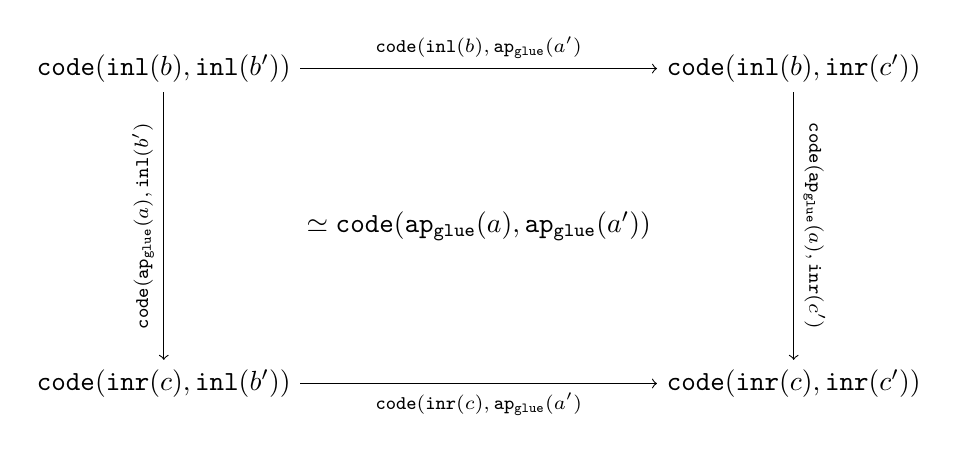
\begin{tikzpicture}
		\node (AA) at (0,0) 
			{ $ \simeq \type{ code } ( \type{ ap_{glue} } ( a ) , \type{ ap_{glue} } ( a' )  )$ }; 
		\node (BB) at (-4,2) 
			{ $ \type{ code } ( \type{ inl } ( b ) , \type{ inl } ( b' )  )$ }; 
		\node (BC) at (4,2) 
			{ $ \type{ code } ( \type{ inl } ( b ) , \type{ inr } ( c' )  )$ }; 
		\node (CB) at (-4,-2) 
			{ $ \type{ code } ( \type{ inr } ( c ) , \type{ inl } ( b' )  )$ }; 
		\node (CC) at (4,-2) 
			{ $ \type{ code } ( \type{ inr } ( c ) , \type{ inr } ( c' )  )$ }; 
		\draw [->] (BB) to 
			node 
				[above] 
				{\scriptsize $ \type{ code } ( \type{ inl } ( b ) , \type{ ap_{glue} } ( a' ) $ } 
			(BC);
		\draw [->] (BB) to 	
			node 
				[rotate=90,above] 
				{ \scriptsize $ \type{ code } ( \type{ ap_{glue} } ( a ) , \type{ inl } ( b' ) $ } 
			(CB);
		\draw [->] (BC) to 
			node 
				[rotate=-90, above] 
				{\scriptsize $\type{ code } ( \type{ ap_{glue} } ( a ) , \type{ inr } ( c' ) $} 
			(CC);
		\draw [->] (CB) to 	
			node 
				[below] 
				{ \scriptsize $ \type{ code } ( \type{ inr } ( c ) , \type{ ap_{glue} } ( a' ) $ } 
			(CC);
	\end{tikzpicture}
\]
Next, let's define all of these elements in this diagram.  
First, we look at the types occupying the corners. 

\vspace{2em}

$\type{ code } \left( \type{ inl } ( b ) , \type{ inl } ( b' ) \right)$ is the most complicated. 
In order to incorporate $\type{ refl }_b$ when $b$ is not in the image of $f$, 
we define this type to be the pushout of the span
\[
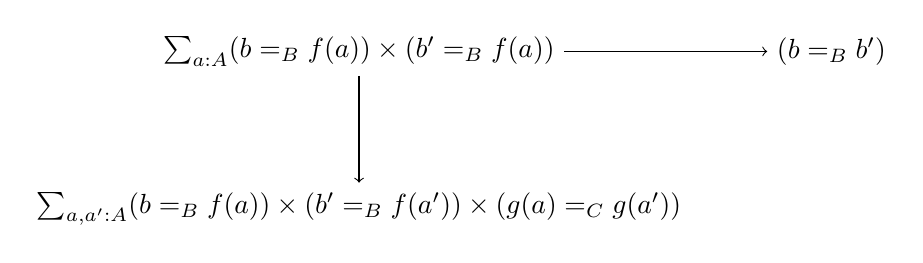
\begin{tikzpicture}
	\node (1) at (0,2) 
		{ $ \sum_{ a : A } ( b =_B f ( a ) ) \times ( b' =_B f ( a ) )  $ };
	\node (2) at (6,2) 
		{ $ ( b =_B b' ) $ };
	\node (3) at (0,0) 
		{ $ \sum_{ a , a' : A } ( b =_B f ( a ) ) \times  (b' =_B f ( a' ) ) \times ( g ( a ) =_C g ( a' ) ) $ };
	\draw [ -> ] (1) to (2);
	\draw [ -> ] (1) to (3);
\end{tikzpicture}
\]
This is a proposition. 
Indeed, the span feet are propositions
and the only way for both to be populated
is if the apex is also populated.
But this would identify the 
left and right included elements
with a glue.

\vspace{2em}

$
\type{ code } \left( \type{ inl } ( b ) , \type{ inr } ( c' ) \right) \coloneqq
	\sum_{ a : A } ( b =_B f ( a ) ) \times ( c' =_C g ( a ) )
$
This is a proposition. 
Indeed, if there does not exist an $ a : A $ such that
$ b =_B f ( a )$ and $ c' =_C g ( a ) $
are both populated, then 
$ \type{ code } \left( \type{ inl } ( b ) , \type{ inr } ( c' ) \right) $ 
is empty. 
If there exists a single $a : A$ such that 
$ b =_B f ( a )$ and $ c' =_C g ( a ) $
are both populated, then 
because they are each equivalent to $ \type{ 1 }$,
$ \type{ code } \left( \type{ inl } ( b ) , \type{ inr } ( c' ) \right) $ 
is also equivalent to $ \type{ 1 }$.
If there is $a, a' : A$ such that
$ b =_B f ( a )$ and $ c' =_C g ( a ) $,
and also 
$ b =_B f ( a' )$ and $ c' =_C g ( a' ) $,
then the injectivity of $f$ and
$f ( a ) =_B b =_B f ( a' )$ 
implies that
$a =_A a'$
which also gives us that 
$ \type{ code } \left( \type{ inl } ( b ) , \type{ inr } ( c' ) \right) $ 
is equivalent to $ \type{ 1 }$.

\vspace{2em}

$
\type{ code } \left( \type{ inr } ( c ) , \type{ inl } ( b' ) \right) \coloneqq
	\sum_{ a : A } ( c =_C g ( a ) ) \times ( b' =_B f ( a ) )
$
This is a proposition by the same sort of argument from above.
	
\vspace{2em}

$
\type{ code } \left( \type{ inr } ( c ) , \type{ inr } ( c' ) \right) \coloneqq
	\sum_{ a , a' : A } ( c =_C g ( a ) ) \times ( c' =_C g ( a' ) ) \times ( f ( a ) =_B f ( a' ) )
$ 	
The injectivity of $f$ gives us that 
	$ f ( a ) =_B f ( a' ) $
imples that 
	$ a =_A a'$
which in turn implies that
	$ g ( a ) =_C g ( a' )$,
hence 
	$ c =_C c'$.
Therefore, 
$
\type{ code } \left( \type{ inr } ( c ) , \type{ inr } ( c' ) \right) =	
	\left( c =_C c'  \right). 
$
Hence 
$ \type{ code } \left( \type{ inr } ( c ) , \type{ inr } ( c' ) \right) $
is a proposition.	

\vspace{2em}

Next, we look at the maps. 
They are all equivalences, hence by univalence
we define them as identity types. 
To show this, we show each is populated.

\vspace{2em}

$ 
\type{ code } \left( \type{ inl } ( b ) , \type{ ap }_{ \type{ glue } } ( a' ) \right) \colon
	\left(
		\type{ code } ( \type{ inl } ( b ) , \type{ inl } ( f ( a' ) ) ) =
		\type{ code } ( \type{ inl } ( b ) , \type{ inr } ( g ( a' ) ) ) 
	\right)
$
Because both sides of the identity type are propositions,
to show that this equivalence holds
it suffices to show that either
$\type{ code } ( \type{ inl } ( b ) , \type{ inl } ( f ( a' ) ) )$
and
$\type{ code } ( \type{ inl } ( b ) , \type{ inr } ( g ( a' ) ) )$
are both empty or both populated.
This follows from post-composition with
$ \type{ glue ( a' ) }$
or its inverse.

\vspace{2em}

$ 
\type{ code } \left( \type{ ap }_{ \type{ glue } } ( a ) , \type{ inl } ( b' ) \right) \colon
	\left(
		\type{ code } ( \type{ inl } ( f ( a ) ) , \type{ inl } ( b' ) ) =
		\type{ code } ( \type{ inr } ( g ( a ) ), \type{ inl } ( b' ) ) 
	\right)
$
This follows from a similar argument to that above, 
with post-composition replaced with pre-composition.

\vspace{2em}

$ 
\type{ code } \left( \type{ inr } ( c ) , \type{ ap }_{ \type{ glue } } ( a' ) \right) \coloneqq
	\left( 
		\type{ code } ( \type{ inr } ( c ) , \type{ inl } ( f ( a' ) ) ) =
		\type{ code } ( \type{ inr } ( c ) , \type{ inr } ( g ( a' ) ) ) 
	\right) 
$ 
This follows from a similar argument.

\vspace{2em}

$ 
\type{ code } \left( \type{ ap }_{ \type{ glue } } ( a ) , \type{ inr } ( c' ) \right) \coloneqq 
	\left( 
		\type{ code } ( \type{ inl } ( f ( a ) ) , \type{ inr } ( c' ) ) =
		\type{ code } ( \type{ inr } ( g ( a ) ) , \type{ inr } ( c' ) ) 
	\right) 
$ 
This follows from a similar argument.

\vspace{2em}

Now we define the $2$-cell to be
\[
	\type{ code } ( \type{ ap }_\type{ glue } ( a ) , \type{ ap }_\type{ glue } ( a' )  ) .
\]
I think this is uniquely determined because
everything involved is a proposition. 
Because we have that the 1-cells 
in the square are equalities,
there is only a single way to commute.
This single way is how we define our 2-cell. 

\textbf{here's a change!!}

\textbf{and another one from amelia!}


%%%%%%%%%%%%%
% end document
%%%%%%%%%%%%%
\end{document}
